\documentclass[aspectratio=169]{beamer}
\usepackage[utf8]{inputenc}
\usepackage{graphicx}
\usepackage{lipsum}

% Theme configuration
\usetheme{CambridgeUS}  % Changed theme from Madrid to CambridgeUS
\usecolortheme{dolphin} % Applied a different color scheme

% Title slide configuration
\title{AKSHARAM}
\subtitle{An Educational Platform for Malayalam Language}
\author{}
\date{}

\begin{document}

% Title Slide
\begin{frame}
    \vspace{1cm}
    \titlepage
    \subtitle
    \vfill
    \begin{columns}[t]
        \begin{column}{0.5\textwidth}
            \begin{flushleft}
                \textbf{Guide Name} \\ 
                Ms. Philo Sumi \\ 
                Assistant Professor\\
                Department of AIDS
            \end{flushleft}
        \end{column}
        \begin{column}{0.5\textwidth}
            \begin{flushright}
            \text {Team Members:}\\  Marc George, Merlin Sarah Jiju, Timon.K.John \\ {Batch No:} 2 \\ {Team No:} 21
            \end{flushright}
        \end{column}
    \end{columns}
\end{frame}

% Contents Slide
\begin{frame}{Contents}
    \begin{enumerate}
        \item Objective
        \item Existing System and its Disadvantages
        \item Proposed System
        \item Advantages of Proposed System
        \item Software / Hardware Requirements
        \item Conclusion
        \item References
    \end{enumerate}
\end{frame}

% Problem Statement Slide
\begin{frame}
    \frametitle{ Problem Statement }
       \tem\textbf{Problem}
       \item Traditional textbook-based learning methods for concepts, subjects, and languages have become increasingly unappealing to modern learners. With the average adult attention span now at just 8.25 seconds, there is a growing demand for faster, more engaging, and cost-effective approaches to language acquisition. In our state, Malayalam remains predominantly taught in conventional classroom settings, limiting accessibility and failing to align with evolving learning preferences.
       \item\textbf{Solution}
       \item To address this challenge, we propose an AI-powered application designed to teach Malayalam from the ground up. The app introduces users to basic characters, progressively building their proficiency in forming and using common Malayalam words. Additionally, it features an image-based text recognition system that scans Malayalam text and translates it into English, enhancing accessibility and learning efficiency.
\end{frame}

% Objective Slide
\begin{frame}{Objective}
    \begin{itemize}
        \item The objective of this project is to develop an AI-powered Malayalam learning platform that enhances language acquisition through interactive experiences.
        \item The system integrates a LeNet-based handwritten character recognition model to assist users in learning how to write Malayalam characters with real-time feedback.
        \item It also provides pronunciation assistance, contextual learning, and conversation-based examples.
        \item The platform employs OCR and a translation model to extract and translate Malayalam text from images.
        \item Additionally, it features a text-to-speech module for accessibility.
    \end{itemize}
\end{frame}

% Existing System Slide
\begin{frame}
    \frametitle{Existing System and its Disadvantages}
    \begin{itemize}
    \end{itemize}
   
   
    \renewcommand{\arraystretch}{1.5} % Increases row height for better spacing
    \setlength{\tabcolsep}{8pt} % Adjusts column spacing for better readability
 % from here----------------------------------------------------------------- 

 \begin{table}[]
        \centering
        \Large % Makes the text larger
        \resizebox{\textwidth}{0.4\textheight}{ % Adjusts height to take up more space
        \begin{tabular}{|p{4cm}|p{6cm}|p{4cm}|p{4cm}|p{4cm}|}
            \hline
            \rowcolor% Adds a light gray background to the header
            \textbf{Title} & \textbf{Summary} & \textbf{Technology Used} & \textbf{Advantages} & \textbf{Disadvantages} \\ \hline
            \textbf Vaisakh V K ,Lyla B Das, \textbf“Handwritten Malayalam Character Recognition System using Artificial Neural Networks”, 2020 & The paper presents a system for recognizing handwritten Malayalam characters using Convolutional Neural Networks (CNN). The process includes image acquisition, preprocessing using OpenCV, segmentation of characters using contour detection, and feature extraction via CNN.  Real-time testing is performed by processing input images and classifying characters into text. & Preprocessing ,Segmentation ,Feature Extraction ,Classification. & Utilizes deep learning for improved performance , Real-time character recognition capability. &  Struggles with variations in individual handwriting styles ,Computationally expensive, requiring powerful hardware, Requires a large labeled dataset for training ,  \\ \hline
        \end{tabular}
        } % End of resizebox
        \caption{Comparison of Existing Systems}
    \end{table}
\end{frame}

\begin{frame}
    \begin{table}[]
        \centering
        \Large % Makes the text larger
        \resizebox{\textwidth}{0.4\textheight}{ % Adjusts height to take up more space
        \begin{tabular}{|p{4cm}|p{6cm}|p{4cm}|p{4cm}|p{4cm}|}
            \hline
            \rowcolor% Adds a light gray background to the header
            \textbf{Title} & \textbf{Summary} & \textbf{Technology Used} & \textbf{Advantages} & \textbf{Disadvantages} \\ \hline
            \textbf Baiju.K.B, Sabna.T.S, Lajish.V.L \textbf"Segmentation of Malayalam Handwritten Characters into Pattern Primitives and Recognition using SVM", 2020 & Proposes a segmentation-based approach for Malayalam handwritten character recognition. Uses RDP and EDFC for segmentation, extracts key features, and classifies using SVM (RBF). & Hi-Tech e-Writemate, Min-Max Normalization, RDP, EDFC, SVM (RBF), Python (Jupyter) . & High accuracy, Efficient feature extraction, Real-time applicability. & Limited to 8 vowels, Requires manual reference set, Struggles with visually similar characters. \\ \hline
             
        \end{tabular}
        } % End of resizebox
        \caption{Comparison of Existing Systems}
    \end{table}
\end{frame}

\begin{frame}
    \begin{table}[]
        \centering
        \Large % Makes the text larger
        \resizebox{\textwidth}{0.4\textheight}{ % Adjusts height to take up more space
        \begin{tabular}{|p{4cm}|p{6cm}|p{4cm}|p{4cm}|p{4cm}|}
            \hline
            \rowcolor% Adds a light gray background to the header
            \textbf{Title} & \textbf{Summary} & \textbf{Technology Used} & \textbf{Advantages} & \textbf{Disadvantages} \\ \hline
            \textbf Manjusha K,Anand Kumar Madasamy,Soman Kp, \textbf"On developing handwritten character image database for Malayalam language script",\textbf 2019 & The paper focuses on developing a handwritten character image database for Malayalam script, essential for research in handwritten text recognition. It presents Amrita MalCharDb, an open-source database containing 85 character classes collected from 77 native Malayalam writers. The database is segmented using active contour models and tested with various feature extraction and classification techniques to evaluate recognition accuracy. & Image Processing ,Feature Extraction ,Classification,Dataset.& Provides a standardized dataset ,High recognition accuracy ,Open-source and extensible for further research. & Computationally expensive feature extraction techniques ,Requires further expansion to include all valid character shapes. \\ \hline
             
        \end{tabular}
        } % End of resizebox
        \caption{Comparison of Existing Systems}
    \end{table}
\end{frame}

\begin{frame}
    \begin{table}[]
        \centering
        \Large % Makes the text larger
        \resizebox{\textwidth}{0.32\textheight}{ % Adjusts height to take up more space
        \begin{tabular}{|p{4cm}|p{6cm}|p{4cm}|p{4cm}|p{4cm}|}
            \hline
            \rowcolor% Adds a light gray background to the header
            \textbf{Title} & \textbf{Summary} & \textbf{Technology Used} & \textbf{Advantages} & \textbf{Disadvantages} \\ \hline
            \textbf Anish S, Preeja V, \textbf“A Novel Method for Malayalam Handwritten Character Recognition”,
            \textbf 2015 & The project focuses on developing an offline handwritten character recognition (HCR) system for the Malayalam language. It employs a texture extraction model using a co-occurrence matrix and Euclidean distance for character identification. & Image Processing: Binarization, Segmentation, Feature Extraction,Classification & High recognition accuracy ,Effective for complex Malayalam characters ,Robust texture-based feature extraction &  Struggles with highly similar characters,Limited to offline recognition ,Requires extensive training data for improved accuracy  \\ \hline
             
        \end{tabular}
        } % End of resizebox
        \caption{Comparison of Existing Systems}
    \end{table}
\end{frame}

\begin{frame}
    \begin{table}[]
        \centering
        \Large % Makes the text larger
        \resizebox{\textwidth}{0.4\textheight}{ % Adjusts height to take up more space
        \begin{tabular}{|p{4cm}|p{6cm}|p{4cm}|p{4cm}|p{4cm}|}
            \hline
            \rowcolor% Adds a light gray background to the header
            \textbf{Title} & \textbf{Summary} & \textbf{Technology Used} & \textbf{Advantages} & \textbf{Disadvantages} \\ \hline
            \textbf Yann LeCun, Leon Bottou, Yoshua Bengio, and Patrick Haffner, \textbf“Gradient Based Learning Applied To Document Recognition”, \textbf 1998 & 
           Discusses the use of multilayer neural networks, especially Convolutional Neural Networks (CNNs), for handwritten character recognition.
           Introduces Graph Transformer Networks (GTN) for training multiple modules in document recognition.
           Demonstrates a CNN-based system for bank check reading deployed commercially.& Neural Networks,Convolutional neural networks(CNN),Graph transformer networks (GNT),Gradient-based learning & High accuracy in handwritten character recognition, reduced need for manual feature engineering,scalable to large datasets and real-world applications. & Requires substantial training data, Computationally expensive, Sensitive to hyperparameter tuning. 
 \\ \hline
             
        \end{tabular}
        } % End of resizebox
        \caption{Comparison of Existing Systems}
    \end{table}
\end{frame}


% Proposed System Slide 1
\begin{frame}
    \frametitle{Proposed System}  
   
    \begin{itemize}
     
        \item  The proposed system aims to assist users in learning Malayalam characters, words, and sentences through AI-powered handwritten character recognition and language translation.
        \item  Utilizes computer vision and optical character recognition technologies to enhance language comprehension by accurately extracting and analyzing Malayalam text and translating it so users can understand.
        \item  Integrates gamification elements such as levels, achievements, and quizzes to make language learning engaging and interactive.
        \item  Focused on usability, accuracy, and accessibility to help learners master Malayalam in an interactive and enjoyable manner.
    \end{itemize}
\end{frame}

% Proposed System Slide 2
\begin{frame}
    \frametitle{Proposed System}
    \begin{itemize}
      \item \textbf{Hand Written Character Recognition}  
        \begin{itemize}
            \item AI model analyzes handwritten Malayalam characters and provides accuracy feedback.
            \item Assists users in improving handwriting through visual guidance and corrections.
        \end{itemize}

        \item \textbf{Malayalam Word Learning }
        \begin{itemize}
            \item Displays Malayalam words and meanings for enhanced vocabulary building.
            \item Provides pronunciation assistance for better spoken language proficiency.
        \end{itemize}

        \item \textbf{Sentence Translation and Contextual Learning}  
        \begin{itemize}
            \item Provides pronunciation assistance for better understanding.
            \item Offers context-based examples to help users understand sentence structures.
        \end{itemize}
        \item \textbf{Image-based Text Recognition}  
        \begin{itemize}
            \item AI-powered OCR extracts Malayalam text from images.
            \item Translates text into English to assist in reading comprehension.
        \end{itemize}
        \item \textbf{Scalability and Adaptability}  
        \begin{itemize}
            \item Suitable for students, language learners, and non-native speakers.
            \item Scalable to incorporate advanced features such as voice recognition and AI-driven personalized learning paths for a more immersive and adaptive learning experience.
        \end{itemize}
        
            
    \end{itemize}
\end{frame}

% Advantages Slide
\begin{frame}
    \frametitle{Advantages of the Proposed System}
    \begin{itemize}
        \item \textbf{User-Friendly and Accesible}     
        \begin{itemize}
            \item  With an intuitive interface, the system is easy to use for learners of all ages and technical expertise.
            
        \end{itemize}

        \item \textbf{Comprehensive Learning Approach}     
        \begin{itemize}
            \item Combining text, images, and handwriting recognition, along with AI-powered pronunciation and contextual learning, it ensures effective comprehension of Malayalam.
            
        \end{itemize}
        \item \textbf{Engaging and Interactive Learning}     
        \begin{itemize}
            \item The system incorporates gamification with levels, achievements, and quizzes to keep learning fun, rewarding, and motivating. 
            
        \end{itemize}
        \item \textbf{Scalability and Future Growth}     
        \begin{itemize}
            \item  Built to scale, the app can expand to include voice recognition and personalized learning paths, with potential support for more languages.
        \end{itemize}
        \item \textbf{Free To Use}     
        \begin{itemize}
            \item The system is completely free, making it accessible to everyone who wants to learn Malayalam without any cost.
        \end{itemize}
    \end{itemize}
\end{frame}

% METHODOLOGY
\begin{frame}{Methodology}
\item \textbf{A. Data Flow Diagrams}
    \begin{figure}
        \centering
        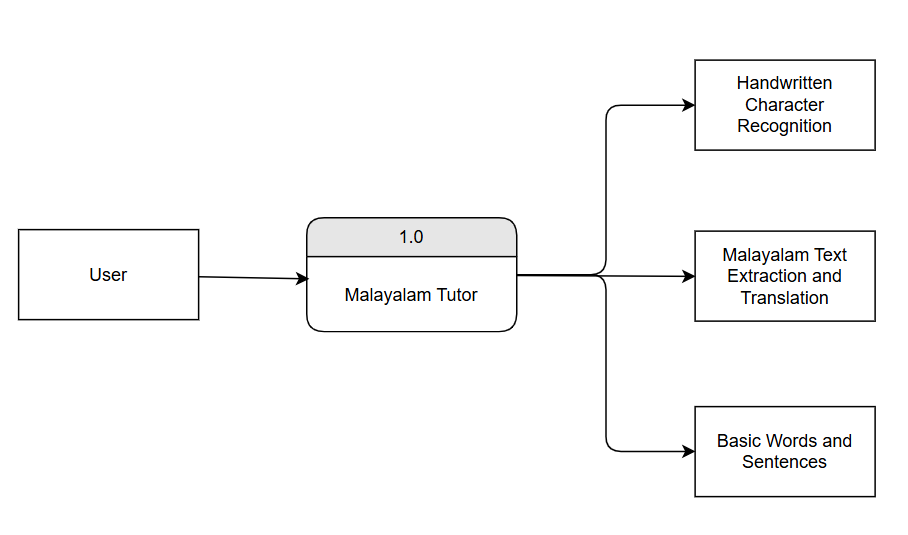
\includegraphics[width=0.7\textwidth]{dfd0.png}
    \end{figure}
\end{frame}
\begin{frame}{Methodology}
\item \textbf{A. Data Flow Diagrams}
    \begin{figure}
        \centering
        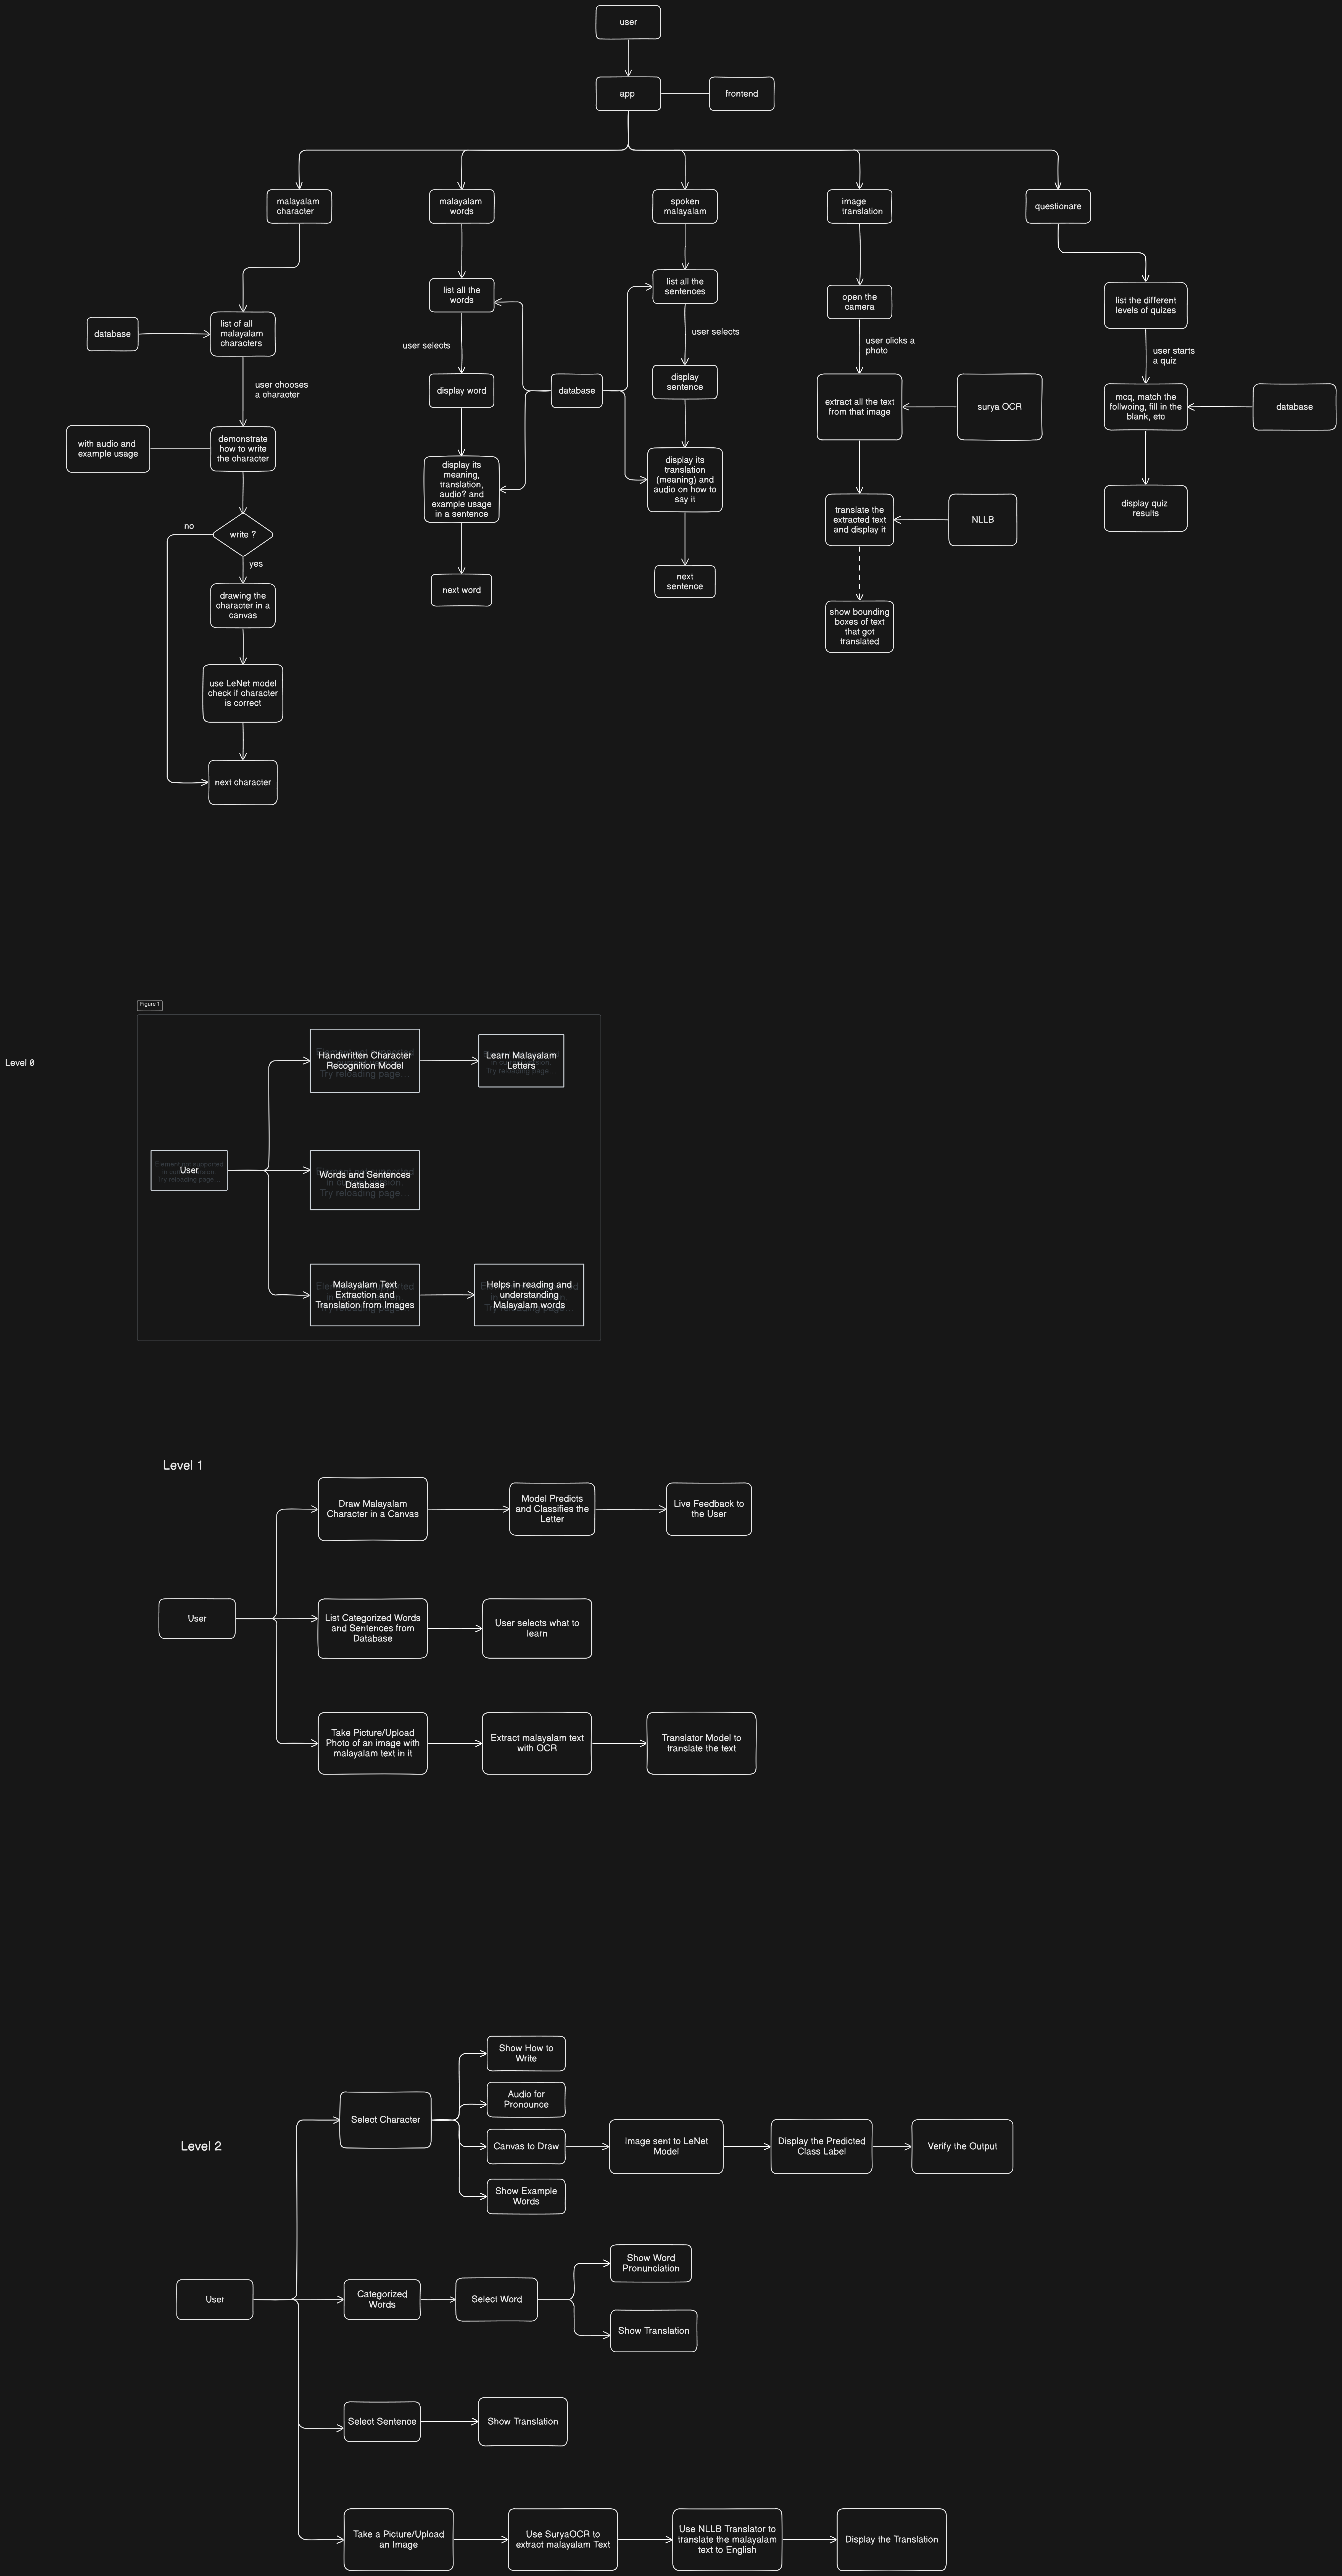
\includegraphics[width=0.7\textwidth]{dfd1.png}
    \end{figure}
\end{frame}
\begin{frame}{Methodology}
\item \textbf{A. Data Flow Diagrams}
    \begin{figure}
        \centering
        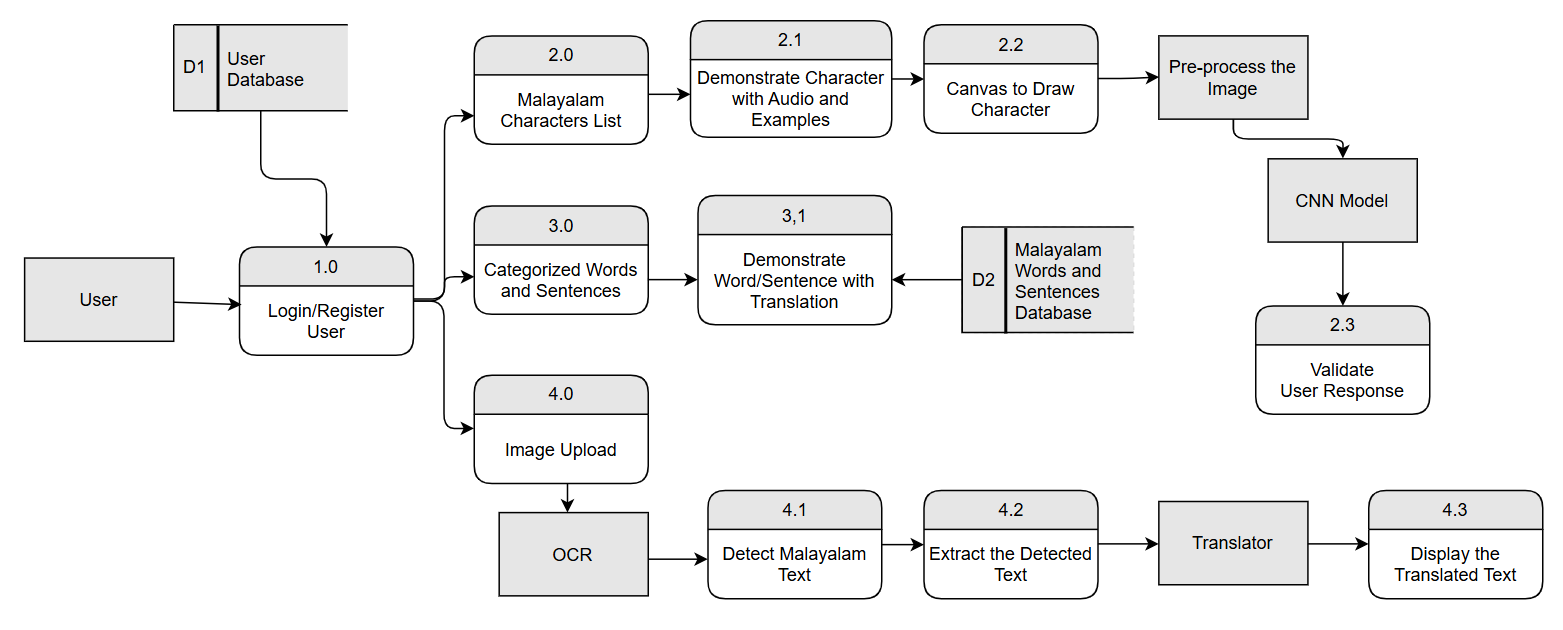
\includegraphics[width=0.5\textwidth]{dfd2.png}
    \end{figure}
\end{frame}

\begin{frame}{Methodology}
\item \textbf{B. Architecture Diagram}
\begin{figure}
        \centering
        \includegraphics[width=0.3\textwidth]{arch.png}
    \end{figure}
\end{frame}
    
% Module Details
\begin{frame}{Methodology}
\item \textbf{C. Module Details}

    \frametitle{Methodolgy}
    \begin{itemize}
        \item\textbf{1. Letter Classification Module: }
            \item The user is shown how to write the character and then their written input is captured in the canvas provided. The image is pre-processed and sent to a classification model, which determines the correct alphabet and decides whether the user can proceed to the next letter.
    \end{itemize}
    \begin{itemize}
            \item \textbf{Components of Letter Classification Module:}
            \item Demo: Demonstrates how to write the letter.
            \item Canvas: The user then writes the letter on the given space.
            \item Classification Model: The written letter is then inputted to the model where it is classified.
            \item Result: Determines whether the user can move on to the next character or not.
        \end{itemize}
\end{frame}

\begin{frame}{Methodology}
\item \textbf{C. Module Details}
    \frametitle{Methodology}
    \begin{itemize}
        \item \textbf{2. Smart Scan Module:}
        \item The Image-Based Learning Module helps users learn Malayalam by extracting and translating text from images. Using an OCR model, the system detects Malayalam words in images, while a translation model converts them into the user's preferred language. This feature enhances learning by providing real-world examples, making language acquisition more interactive and engaging.
        \item \textbf{Components of Smart Scan Module:}
        \item Image Input: Users upload or capture an image containing Malayalam text.
        \item OCR Model: Extracts Malayalam words from the image.
        \item Translation Model: Translates the extracted text into the desired language.
        \item Result: Shows the original and translated text for learning.
    \end{itemize}
\end{frame}

\begin{frame}{Methodology}
\item \textbf{C. Module Details}
    \frametitle{Methodology}
    \begin{itemize}
        \item \textbf{3. Words and Sentences Learning Module:}
        \item Helps users build their Malayalam vocabulary and conversational skills using a structured database. It teaches Malayalam words by displaying their meanings, pronunciation. Additionally, it introduces basic Malayalam sentences providing example sentences along with its English translations to enhance understanding and fluency.
        \item \textbf{Components of Words and Sentences Learning Module:}
        \item Demo: Shows the word and sentence along with its pronunciation and translation.
        \item 
    \end{itemize}
\end{frame}

% Software / Hardware Requirements Slide
\begin{frame}
    \item \textbf{Software Requirements}     
        \begin{itemize}
            \item Pytorch - For the handwritten Character recognition model and translator model. 
            \item SuryaOCR - For Optical Character Recognition of Malayalam Words. 
            \item OpenCV - For Preprocessing images. 
            \item Django - For the backend of the platform.
            \item ReactJS - For an interactive and user friendly frontend application.
        \end{itemize}
\end{frame}

% Pending Tasks
\begin{frame}{Pending Tasks}
    \begin{itemize}
        \item \textbf{Frontend:} Develop and implement the user interface, ensuring a responsive and intuitive design for seamless user interaction.
        \item \textbf{Letter Classificaton Model Optimization:} Trying to achieve better accuracy for the test results and how to optimize the model.
    \end{itemize}
\end{frame}

% Conclusion Slide
\begin{frame}
    \frametitle{Conclusion}
    \begin{itemize}
       \item In conclusion, the proposed AI-powered Malayalam learning platform utilizes advanced handwritten character recognition and OCR-based text extraction to enhance the language learning experience.
       \item By leveraging AI-driven translation and pronunciation assistance, the system provides users with a structured and interactive way to learn Malayalam characters, words, and sentences.
       \item Additionally, the platform facilitates contextual learning by offering real-world usage examples, helping users grasp the language more effectively .
       \item This project not only promotes efficient self-paced learning but also encourages linguistic and cultural awareness, making Malayalam more accessible to a broader audience.
       \item With its scalable and intelligent approach, the platform serves as an innovative solution to modern language learning challenges, bridging the gap between traditional and AI-powered education.
       
    \end{itemize}
\end{frame}

% References Slide
\begin{frame}
    \frametitle{References}
    \begin{itemize}
 \item Vaishakh.V.K ,Lyla.B.Das, “Handwritten Malayalam Character Recognition System using Artificial Neural Networks”, 2020.
 \item Baiju.K.B ,Sabna.T.S, Lajish.V.L, “Segmentation of Malayalam Handwritten Characters into Pattern Primitives and Recognition using SVM”, 2020.
 \item P Shourie, V Anand, D Upadhyay, "On developing handwritten character image database for Malayalam language script", 2019.
  \item Yann Le-
Cun, Leon Bottou,Yoshua Bengio, and Patrick Haffner, "Gradient Based Learning Applied To Document Recognition", 1998.
 \item Dzmitry Bahdanau, KyungHyun Cho, Yoshua Bengio, 'Neural machine translation by jointly learning to align and translate', 2014.
    \end{itemize}
\end{frame}

% Thank You Slide
\begin{frame}
    \begin{center}
        \Large \textbf{Thank You!}
    \end{center}
\end{frame}

\end{document}
